\section{Evaluation}\label{experiments}
We evaluate our models on the ACE 2005 corpus to investigate the following questions: (1) can our neural network models achieve
satisfactory performances without feature engineering; (2) can our models alleviate the language issue in Chinese event extraction?

\subsection{Experimental Setup}
\paragraph{Dataset and evaluation methodology}
We used the standard ACE 2005 corpus in our evaluation, which contains 633 Chinese documents. Unlike English, the ACE Chinese corpus does not have a recognized partition of documents for evaluation. Most of the previous work \cite{chen2009language,feng2016language} randomly select about 10\% of the 633 documents as the test set. However, as reported by Chen and NG \shortcite{chen2012joint} via 10-fold cross validation, performances achieved on different partitions vary considerably due to the small size of test sets. Therefore, cross validation may be a better choice when conducting experiments on the ACE 2005 corpus. In order to make accurate evaluation and save time, we perform 5-fold cross-validation and report our performances averaged over five folds.

\paragraph{Evaluation measures} Similar to previous work, we evaluated our models in terms of $precision (P)$, $recall (R)$, and $F{-}measure (F)$ for each subtask. These performance metrics are computed according to the following standards of correctness for four subtasks:
\begin{itemize}	
	\item For trigger identification, a trigger is correctly identified if its offsets exactly match a reference trigger;
	\item For trigger classification, a trigger is correctly classified if its trigger type and offsets exactly match a reference trigger;
	\item For argument identification, an argument is correctly identified if its offset, related trigger type and trigger’s offsets exactly match a reference argument;
	\item For argument classification, an argument is correctly classified if its offsets, role, related trigger type and trigger’s offsets exactly match a reference argument.
\end{itemize}

\subsection{Network Training}
\paragraph{Parameter initialization} All matrix parameters (including weight matrices in neural network layers and
transition matrix in the CRF layer) are randomly initialized with uniform samples from range
$[-\sqrt{\frac{6}{row+col}}, +\sqrt{\frac{6}{row+col}}]$, where $row$ and $col$ are the number of rows and columns in
the matrix \cite{glorot2010understanding}. Bias vectors are initialized to zero.

\paragraph{Pre-trained embeddings} Initializing word vectors with those obtained from a neural language model is a
popular method to improve performance in the absence of a large training set. \cite{collobert2011natural}. Both word
and character embeddings are trained on over 261 thousand articles crawled from Chinese news website, using skip-gram
word2vec model \cite{mikolov2013distributed}. All embeddings are fine tuned during training.

\paragraph{Optimization algorithm} All models share a generic stochastic gradient descent (SGD) forward and backward
training procedure. For all models presented, parameter optimization is performed using Adam \cite{kingma2014adam} with
gradient clipping \cite{pascanu2013difficulty}. We also apply the dropout method \cite{srivastava2014dropout} on both
the input and output vectors of all models to mitigate overfitting.

\paragraph{Hyper-parameters} In different stages of event extraction, we adopted different parameters.
Table~\ref{eight} summarizes the chosen hyper-parameters for all experiments.

\begin{table}
\tbl{Hyper-parameters for all experiments.\label{eight}}
  {\begin{threeparttable}
\begin{tabular}{llp{0.25\columnwidth}p{0.25\columnwidth}} \toprule
	\textbf{Layer} & \textbf{Hyper-parameter} & \textbf{Trigger identification and classification} & \textbf{Argument identification and classification} \\
    \midrule
	\rowcolor{Gray} & word embedding & \cellcolor{Gray}200 & -- \\
    \rowcolor{Gray} \textbf{Input} & character embedding & 100 & 100 \\
    \rowcolor{Gray} & feature embedding{$^1$} & -- & 32 \\
	 \textbf{Dropout} & dropout rate & 0.5 & 0.5 \\
	\rowcolor{Gray} \textbf{GRU} & state size & 100 & 100 \\
	\multirow{3}{*}{\textbf{CNN}} & context size & 7 & sentence length \\ & kernel sizes & [2, 4, 6] & [1, 2, 3, 4, 5] \\ & number of filters & [32, 32, 32] & [16, 16, 16, 16, 16] \\
    \bottomrule
\end{tabular}
\begin{tabnote}%
\tabnoteentry{$^1$}{Feature embeddings, including trigger position embedding, trigger type embedding, argument position embedding and entity type embedding, have the same size.}
\end{tabnote}%
\end{threeparttable}}
\end{table}

\subsection{Compare with State-of-the-art Methods}
Table~\ref{tab:two} shows the overall performance of all methods on the ACE2005 Chinese corpus. We select the following state-of-art methods for comparison.

\begin{itemize}
	\item \textbf{Char-MEMM} \cite{chen2009language} is the first character-based method to handle the language specific issues, which trains a Maximum Entropy Markov Model to label each character with BIO tagging scheme.
	\item \textbf{Rich-L} \cite{chen2012joint} is a joint-learning, knowledge-rich approach that extends the union of the features employed by Char-MEMM and Li et al. \shortcite{li2012employing} with six groups of linguistic features, including character-based features and discourse consistency features, which is the feature-based state-of-art system.
	\item \textbf{HNN} \cite{feng2016language} is a hybrid neural network model, which also incorporates both bidirectional LSTMs and convolutional neural networks to capture sentence and structure semantic information, and it achieves state-of-the-art performance in Chinese event detection.
\end{itemize}

%Table
\begin{table}%
\newcommand{\tabincell}[2]{\begin{tabular}{@{}#1@{}}#2\end{tabular}}
\tbl{Overall system performance (\%)\label{tab:two}}{
\begin{tabular}{|l|c|c|c|c|c|c|c|c|c|c|c|c|} \hline
	\multirow{2}{*}{\textbf{Model}} &
	\multicolumn{3}{c|}{\tabincell{c}{\textbf{Trigger} \\ \textbf{Identification}}} &
	\multicolumn{3}{c|}{\tabincell{c}{\textbf{Trigger} \\ \textbf{Classification}}} &
	\multicolumn{3}{c|}{\tabincell{c}{\textbf{Argument} \\ \textbf{Identification}}} &
	\multicolumn{3}{c|}{\tabincell{c}{\textbf{Argument} \\ \textbf{Classification}}} \\
	\cline{2-13}
	& P & R & F & P & R & F & P & R & F & P & R & F \\ \hline
	\rowcolor{Gray} Char-MEMM & \bf 82.4 & 50.6 & 62.7 & \bf 78.8 & 48.3 & 59.9 & \bf 64.4 & 36.4 & 46.5 & \bf 60.6 & 34.3 & 43.8 \\ \hline
	Rich-L & 62.2 & \bf 71.9 & 66.7 & 58.9 & \bf 68.1 & 63.2 & 43.6 & \bf 57.3 & 49.5 & 39.2 & \bf 51.6 & 44.6 \\ \hline
	\rowcolor{Gray} HNN & 74.2 & 63.1 & \bf 68.2 & 77.1 & 53.1 & 63.0 & \multicolumn{6}{|c|}{\cellcolor{Gray}--} \\ \hline \hline
	C-BiLSTM$_{word}$ & 65.2 & 62.7 & 63.9 & 61.7 & 59.4 & 60.5 & 50.3 & 50.2 & 50.2 & 43.4 & 43.3 & 43.3 \\ \hline
	\rowcolor{Gray} \quad + Errata table & 68.3 & 65.8 & \bf 66.9 & 62.7 & 60.9 & 61.6 & 49.2 & 52.1 & 50.6 & 42.4 & 44.8 & 43.5  \\ \hline
	C-BiLSTM$_{char}$ & 63.7 & 63.2 & 63.4 & 60.1 & 59.6 & 59.9 & 49.8 & 52.8 & 51.2 & 42.4 & 45.0 & 43.6  \\ \hline
	\rowcolor{Gray} \quad + Errata table & 67.0 & 66.4 & 66.7 & 60.7 & 62.6 & 61.5 &  49.8 & 53.0 & 51.2 & 42.8 & 45.5 & 44.1  \\ \hline
	C-BiLSTM-CRF$_{char}$ & 66.1 & 67.9 & \bf 66.9 & 62.5 & 64.2 & \bf 63.3 &  50.8 & 54.1 & \bf 52.4 & 44.0 & 46.8 & \bf 45.3 \\ \hline
\end{tabular}}
\end{table}

Our reported results are averaged over five folds. We directly list the results of previous work from their paper. Although they all evaluated on ACE 2005 corpus, only Rich-L performs cross validation, while Char-MEMM and HNN select their test set randomly, therefore it is inappropriate to compare their performances directly.

\paragraph{Comparison with Char-MEMM} Char-MEMM concludes that \emph{neighborly word features} are fairly applicable. They utilize the left word and right word of an entity to reduce spurious argument, which is similar to the motivation of our CNN-extracted lexical features. They obtain the highest precisions but lowest recalls on all subtasks. However, all neural network models outperforms in F1 on the first three subtasks. Because neural network methods can avoid the errors propagating from other NLP tools like dependency parsing and POS tagging, while capturing not only neighborly word features but also sentence-level information in the absence of feature engineering.

\paragraph{Comparison with Rich-L} Our best model is a character-based C-BiLSTM-CRF model, and it outperforms Rich-L on both trigger labeling and argument labeling. Note that in argument labeling, some of the arguments are not in the same sentence with their triggers. It is a bottleneck of our C-BiLSTM model, while Rich-L uses discourse-level features to deal with this problem. Under this unfavorable circumstance, our C-BiLSTM can still achieve a better performance against Rich-L, which depends on sophisticated human designed features.

\paragraph{Comparison with HNN} It is not appropriate for us to directly compare our results with this model, as it evaluates on randomly selected test documents. Our C-BiLSTM model assembles HNN model in the choice of neural networks, since both of them concatenate the output vector of BiLSTM and CNN, but their CNN parts and final outputs are different in two aspects. CNN in C-BiLSTM learns a representation over shallow windows for every word, rather than the entire sentence as in HNN model. We argue that C-BiLSTM can obtain more accurate contextual information, because different words may have different context, and, as a result, should have different contextual feature representations instead of sharing one sentence level representation. Moreover, HNN treats event detection as a classification task that determine whether each word is an event trigger, so it can not identify neither inside-word nor cross-word triggers.

\subsection{Word-based C-BiLSTM vs. Character-based C-BiLSTM}
As shown in Table~\ref{tab:two}, when applying the same network architecture to the same subtask, word-based methods always have higher precisions while character-based methods always have higher recalls.

\begin{table}
\newcommand{\tabincell}[2]{\begin{tabular}{@{}#1@{}}#2\end{tabular}}
\tbl{Performance of different types of triggers by different models on trigger labeling.{$^2$}\label{tab:three}}{
\begin{tabular}{|l|l|p{0.6cm}<{\centering}|p{0.6cm}<{\centering}|p{0.6cm}<{\centering}|p{0.6cm}<{\centering}|p{0.6cm}<{\centering}|p{0.6cm}<{\centering}|p{0.6cm}<{\centering}|p{0.6cm}<{\centering}|p{0.6cm}<{\centering}|} \hline
\multirow{2}{*}{\textbf{Stage}} & \multirow{2}{*}{\textbf{Model}} &
\multicolumn{3}{c|}{\textbf{Regular Triggers}{$^1$}} & \multicolumn{3}{c|}{\textbf{Inside-word Triggers}} & \multicolumn{3}{c|}{\textbf{Cross-word Triggers}} \\ \cline{3-11}
 & & P & R & F & P & R & F & P & R & F \\ \hline
\rowcolor{Gray}
    & C-BiLSTM$_{word}$ & 64.1 & 72.4 & 68.0 & -- & 0 &  -- & 63.0 & 44.6 & \bf 52.3 \\ \cline{2-11}
\rowcolor{Gray} & C-BiLSTM$_{char}$ & 67.6 & 68.5 & 68.0 & 20.3 & 30.8 & 37.6 & 57.8 & 31.2 & 40.5 \\ \cline{2-11}
\rowcolor{Gray} \multirow{-3}{*}{\tabincell{l}{\cellcolor{Gray}Trigger \\ \cellcolor{Gray}Identification}} & C-BiLSTM-CRF$_{char}$ & 67.6 & 72.4 & \bf 70.0 & 51.1 & 40.7 & \bf 45.3 & 51.3 & 38.9 & 44.3 \\ \hline
\multirow{3}{*}{\tabincell{l}{Trigger \\ Classification}}
& C-BiLSTM$_{word}$ & 60.6 & 68.4 & 64.2 & -- & 0 & -- & 57.8 & 40.9 & \bf 47.9 \\ \cline{2-11}
& C-BiLSTM$_{char}$ & 64.1 & 64.9 & 64.5 & 18.0 & 27.3 & 21.7 & 49.7 & 26.8 & 34.9 \\ \cline{2-11}
& C-BiLSTM-CRF$_{char}$ & 64.0 & 68.5 & \bf 66.2 & 46.7 & 37.2 & \bf 41.4 & 47.8 & 36.2 & 41.2 \\ \hline
\end{tabular}}
\begin{tabnote}
\tabnoteentry{$^1$}{We regard regular triggers as triggers composed of exactly one word.}
\tabnoteentry{$^2$}{We use NLPIR to perform word segmentation, and the number of regular triggers, inside-word triggers and cross-word triggers are 2863, 172 and 298, respectively.}
\end{tabnote}
\end{table}

We then take a further step to investigate their impacts on different kinds of triggers. As shown in Table~\ref{tab:three} that:

\begin{enumerate}
	\item Both character-based and word-based methods achieve similar performances in regular trigger identification, and character-based method performs slightly better in trigger classification, 0.3\% higher than word-based method in F-measure;
	\item Word-based methods can not label inside-word triggers, while character-based methods can handle this issue, which brings higher overall recall;
	\item It is more difficult for character-based method to correctly identify cross-word triggers. As there are more cross-word triggers than inside-word triggers in dataset, the overall F-measure of word-based methods is slightly higher.
\end{enumerate}

\begin{table}
\newcommand{\tabincell}[2]{\begin{tabular}{@{}#1@{}}#2\end{tabular}}
\tbl{Error analysis: examples of triggers mislabeled by character-based C-BiLSTM.\label{tab:five}}{
\begin{tabular}{p{0.25cm}llp{0.6cm}l}\toprule
\multicolumn{2}{l}{\textbf{Sentence}} & \textbf{Triggers} & \multicolumn{2}{l}{\textbf{Labels}} \\ \midrule
\rowcolor{Gray} S9: & \textbf{走访} 相关 人员 以后,...
& 走访  & expect: & \texttt{BI} \\
\rowcolor{Gray} & After \textbf{visiting} to relevant staff, ... & visiting & output: &\texttt{BO} \\

S10: & \textbf{贺电} 全文 如下:
& 贺电 & expect: & \texttt{BI} \\
& There is the full \textbf{congratulatory message} & congratulatory message & output: & \texttt{OB} \\

\rowcolor{Gray}S11: & 小偷 被 逼 进 \textbf{死 胡同}。& 死 胡同 & expect: & \texttt{O OO} \\
\rowcolor{Gray} & The thief was chased into a \textbf{dead end}. & dead end & output: & \texttt{B OO} \\ \bottomrule
\end{tabular}}
\end{table}

We find several reasons that cause the lower precision of character-based method:

\begin{enumerate}
	\item Character-based method needs to learn the basic patterns of word segmentation by itself. 8.7\% triggers identified by character-based method are partially mislabeled into inside-word triggers, like triggers in S9 and S10,  which leads to a low level precision for inside-word triggers labeling.
	\item Word embedding brings richer semantic information than character embedding. Take S11 in Table~\ref{tab:five} as an example, characters ``胡'' and ``同'' do not have any meaning related to the formed word ``胡同'' (alleyway), while this word strongly suggests that ``死'' (dead) is not a trigger within the context ``死胡同'' (dead end). Given the more accurate embedding of surrounding context, word-based networks can understand the meaning of the center word thus lead to better disambiguation.
	\item GRU units in character-based method needs to maintain clues for longer sequences, as 1.6 times longer than the average length of word sequences. In trigger classification, when we evaluate on sentences containing more than 100 characters, F-measure of character-based method is 57.3\%, while word-based method can achieve 59.8\%, suggesting that GRU units lose some information for longer sequences.
\end{enumerate}

\subsection{Neural Network Architectures}
To compare the effectiveness of different neural network components of C-BiLSTM, we detect events by using BiLSTM and CNN separately. As Table~\ref{tab:four} shows, BiLSTM is more efficient than CNN, especially in argument labeling. And the combined C-BiLSTM model outperforms all other models on all subtasks. This observation demonstrates that \textbf{both of the BiLSTM and CNN models are important for event extraction, and have certain complementarity with each other.}

\begin{table}
\newcommand{\tabincell}[2]{\begin{tabular}{@{}#1@{}}#2\end{tabular}}
\tbl{Comparison of performances of BiLSTM, CNN and C-BiLSTM model. Performances of argument labeling are evaluated on gold standard event triggers. \label{tab:four}}{
\begin{tabular}{|l|p{0.6cm}<{\centering}|p{0.6cm}<{\centering}|p{0.6cm}<{\centering}|p{0.6cm}<{\centering}|p{0.6cm}<{\centering}|p{0.6cm}<{\centering}|p{0.6cm}<{\centering}|p{0.6cm}<{\centering}|p{0.6cm}<{\centering}|p{0.6cm}<{\centering}|p{0.6cm}<{\centering}|p{0.6cm}<{\centering}|} \hline
\multirow{2}{*}{\textbf{Model}} &
\multicolumn{3}{c|}{\tabincell{c}{\textbf{Trigger} \\ \textbf{Identification}}} &
\multicolumn{3}{c|}{\tabincell{c}{\textbf{Trigger} \\ \textbf{Classification}}} \\ \cline{2-7}
& P & R & F & P & R & F \\ \hline
\rowcolor{Gray} BiLSTM$_{word}$ & 66.0 & 59.7 & 62.7 & 59.3 & 60.1 & 59.5 \\ \hline
CNN$_{word}$ & 67.6 & 58.2 & 62.5 & 63.8 & 54.9 & 59.0 \\ \hline
\rowcolor{Gray} C-BiLSTM$_{word}$ & 65.2 & 62.8 & 63.9 & 61.7 & 59.4 & 60.5 \\ \hline \hline
\multirow{2}{*}{\textbf{Model}} &
\multicolumn{3}{c|}{\tabincell{c}{\textbf{Argument} \\ \textbf{Identification}}} &
\multicolumn{3}{c|}{\tabincell{c}{\textbf{Argument} \\ \textbf{Classification}}} \\ \cline{2-7}
& P & R & F & P & R & F \\ \hline
\rowcolor{Gray} BiLSTM$_{char}$ & 68.7 & 73.4 & 71.0 & 60.4 & 64.5 & 62.4 \\ \hline
CNN$_{char}$ & 67.1 & 66.9 & 66.9 & 60.4 & 60.2 & 60.3  \\ \hline
\rowcolor{Gray} C-BiLSTM$_{char}$ & 69.5 & 74.4 & 71.9 & 61.3 & 65.6 & 63.4  \\ \hline
\end{tabular}}
\end{table}

Another challenge here is that some words can trigger different types of events, given different contexts. Take S12 and S13 for example, the word ``释放'' (released) in S12 means releasing gas and expresses an $Attack$ event, while in S13, it means setting somebody free. These ambiguous words account for 36.8 percent of all triggers. We further evaluate the capacity of each network on ambiguous triggers.

\begin{quote}
	S12: 部队 向 抗议者 \textbf{释放} 了 催泪弹 。
	
	\hspace{0.75cm} The troops \textbf{released} tear gas to the protesters.
	
	\hspace{0.75cm} [type: \emph{attack}]
\end{quote}

\begin{quote}
	S13: 他 在 服刑 五 年 后 从 狱中 \textbf{释放} 出来 。
	
	\hspace{0.75cm} He was \textbf{released} from prison after serving a sentence of five years.
	
	\hspace{0.75cm} [type: \emph{release-parole}]
\end{quote}

\begin{table}
\tbl{Percentages of ambiguous words classified correctly. All networks listed in this table are word-based.\label{tab:six}}{
\begin{tabular}{lccc} \toprule
 & \textbf{BiLSTM} & \textbf{CNN} & \textbf{C-BiLSTM} \\ \midrule
    ambiguous word classification ($\%$) & 61.4 & 61.7 & 64.1 \\
 \bottomrule
\end{tabular}}
\end{table}

Table~\ref{tab:six} provides evidences that, benefited from the salient local contextual features, CNN can performs better than BiLSTM on ambiguous triggers, while BiLSTM-extracted sentence-level information also help reduce some errors caused by ambiguous triggers. C-BiLSTM model that combines both levels of features, achieve highest precision as we expected.

\subsection{C-BiLSTM vs. C-BiLSTM-CRF}

\begin{figure}
	\centering
	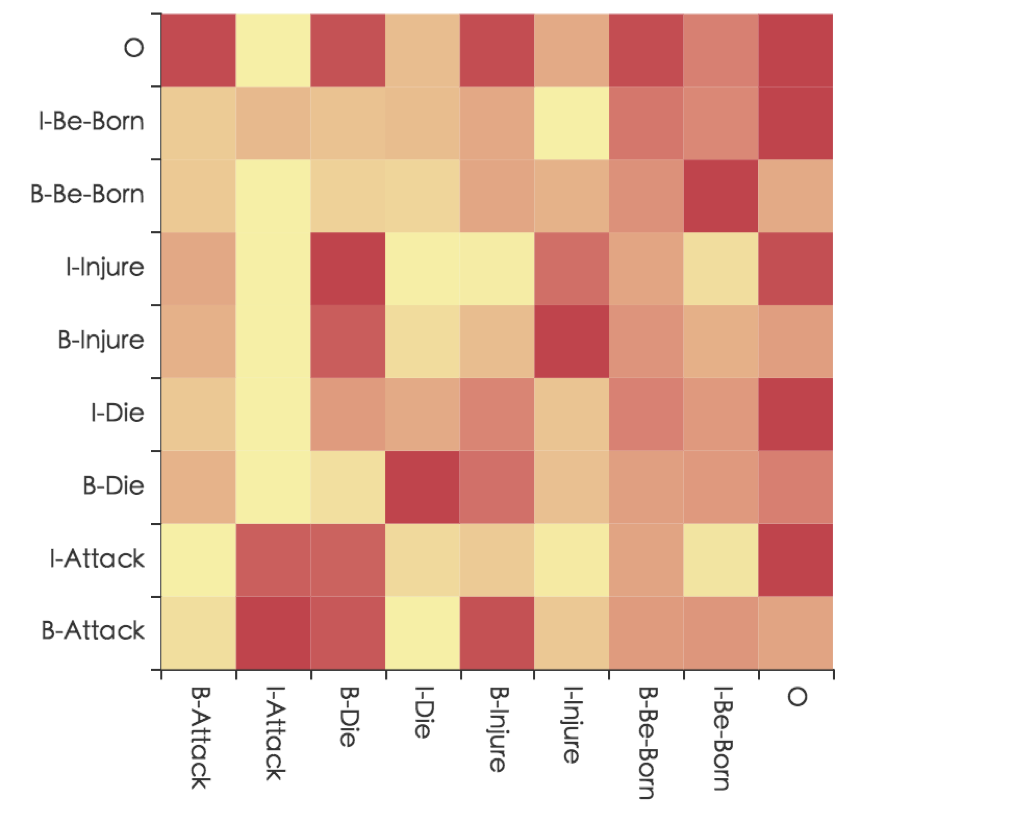
\includegraphics[width=.5\textwidth]{CRF.png}
	\caption{A visualization of a submatrix of transition score in CRF layer. The horizontal axis represents label of current word and the vertical axis represents label of previous word. The darker the color, the higher the score.}
	\label{figure3}
\end{figure}

In Table~\ref{tab:two}, we can see that our character-based convolution BiLSTM-CRF model significantly outperforms other state-of-the-art methods. We list the performance on different types of triggers by C-BiLSTM-CRF and C-BiLSTM model in Table~\ref{tab:three}. Compared with C-BiLSTM models, instead of modeling tagging decisions independently, C-BiLSTM-CRF model takes into account the correlations between labels, which contributes to a 2\% increase of F1 in regular trigger identification, and a 7.7\% increase of F1 in inside-word trigger identification.
We select a subset of labels and generate a heat map in Figure~\ref{figure3} from the transition scores between each label. We find that the better performance of C-BiLSTM-CRF model can be further explained by the following two reasons:
\begin{enumerate}
	\item A CRF layer characterizes the constraints nicely: for a specific event type \texttt{Type}, \texttt{I-Type} can only follow \texttt{B-Type} or \texttt{I-Type}. In other words, if the current label is \texttt{I-Type}, the transition scores for previous labels, except \texttt{B-Type} and \texttt{I-Type}, are invalid and supposed to be very low. For example, as the forth column shows, going from \texttt{B-Die} or \texttt{I-Die} to \texttt{I-Die} is encouraged, while other transitions, like \texttt{B-Attack} to \texttt{I-Die} or \texttt{I-Injure} to \texttt{I-Die} are discouraged.
	\item A CRF layer models the co-occurrences of several event types. For example, an \emph{Attack} event is usually followed by an \emph{Injure} event or a \emph{Die} event. As a result, in the first row, the transition scores of going from \texttt{B-Attack} to \texttt{B-Injure} or \texttt{B-Die} are much higher than other labels start with \texttt{B-}, such as \texttt{B-Be-born}.
\end{enumerate}

Figure~\ref{figure43} shows the whole transition matrix after training. The darkest color grids always appear right below the diagonal, which suggests that for a given label \texttt{B-type}, its most likely following label is \texttt{I-Type}. As we can conclude from Figure~\ref{figure4}, during training, CRF layer gradually learns a score for going from one label to another label and encourages valid paths of labels, while discouraging other invalid or unusual paths.

\begin{figure}
\centering
\subfigure[Initial transition matrix]{\label{figure41} 
\includegraphics[width=0.32\textwidth]{CRF2}}
\subfigure[Epoch=5]{\label{figure42} 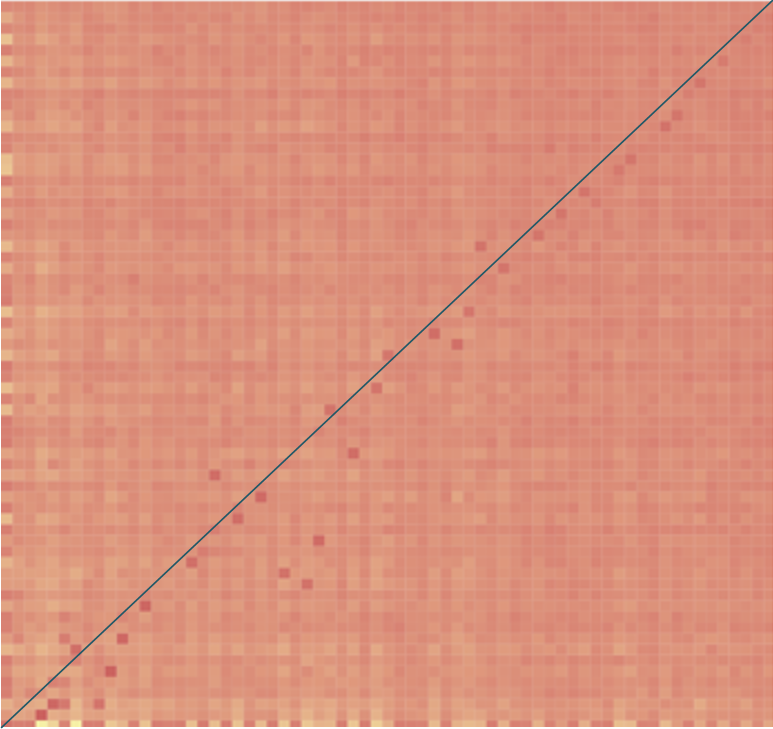
\includegraphics[width=0.32\textwidth]{CRF3}}
\subfigure[Epoch=10]{\label{figure43} 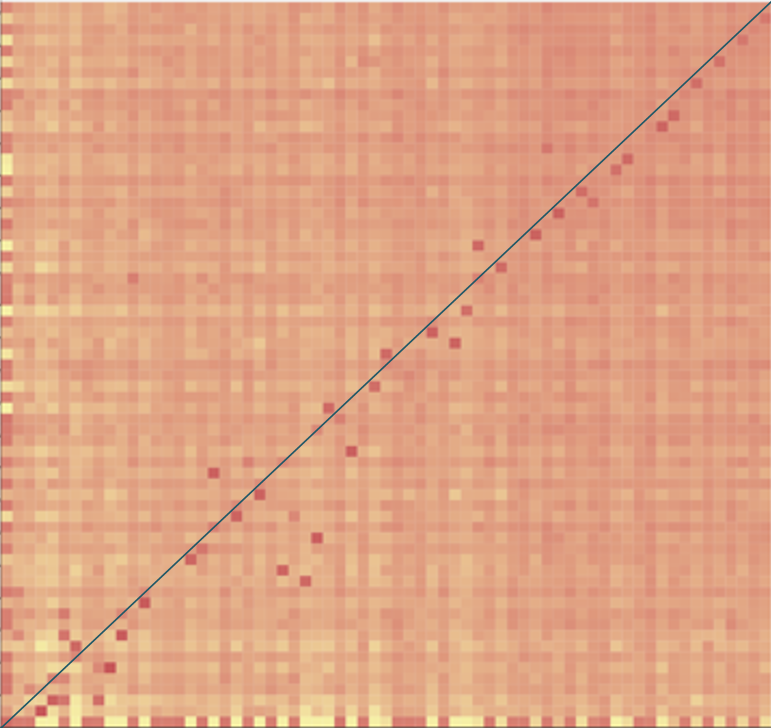
\includegraphics[width=0.32\textwidth]{CRF4}}
\caption{Transition score matrix in CRF layer during training, visualized with heatmaps. Axes have the same meaning as Figure~\ref{figure3}: the horizontal axis represents label of current word while the vertical axis represents label of previous word. Labels in both axes are arranged by their types in the same order as Figure~\ref{figure3}, i.e., \texttt{O, B-type1, I-type1, B-type2, I-type2, B-type3, ...}}
\label{figure4}
\end{figure}
